\chapter{\IfLanguageName{dutch}{Proof of concept en praktijktest}{Proof of concept and field tests}}
\label{ch:poc}
Na de literatuurstudie, requirementsanalyse en vergelijkende evaluatie van bestaande AI-systemen, vormt dit hoofdstuk een belangrijke schakel in het beantwoorden van de centrale onderzoeksvraag. Hierin wordt het geselecteerde AI-systeem geïmplementeerd in een reële context bij volleybalclub Lindemans Aalst als een proof of concept (PoC).

Deze fase heeft tot doel om de theoretische meerwaarde van het systeem in de praktijk te valideren. Tijdens trainingen en wedstrijden wordt geëvalueerd of het systeem voldoet aan de functionele en technische vereisten zoals geformuleerd in de voorgaande fases. Hierbij wordt bijzondere aandacht besteed aan de gebruiksvriendelijkheid, de nauwkeurigheid van dataverzameling, de snelheid van verwerking en de integratie in de bestaande werkwijze van de club.

Het oorspronkelijke plan voorzag een praktijktestperiode van twee weken. Echter, aangezien het volleybalseizoen onverwacht tot een einde kwam tijdens het midden van deze fase, kon de proof of concept slechts tijdens twee resterende wedstrijden worden uitgevoerd. Ondanks deze beperkte testperiode bood dit toch waardevolle inzichten in de toepasbaarheid en prestaties van het AI-systeem in een wedstrijdcontext.

Door de prestaties van het geautomatiseerde systeem te vergelijken met handmatig geregistreerde gegevens en door feedback van coaches en staf te verzamelen, wordt nagegaan of het AI-systeem daadwerkelijk een significante meerwaarde kan bieden voor de werking van de club. De inzichten uit deze praktijktest vormen een essentiële basis voor het formuleren van aanbevelingen omtrent een bredere implementatie op lange termijn.

In bijlage \ref{ch:afkortingen} is een overzicht te vinden van de afkortingen die in dit hoofdstuk worden gebruikt. De andere statistieken en vergelijkingen zijn te vinden in bijlage \ref{ch:statistieken}.

\section{Kwartfinale Play-offs - 16/4/2025}
\subsection{Vergelijking van de statistieken}
\subsubsection{Set 2 - Lindemans Aalst}
\label{sec:PL1_Aalst2}
In de tabellen \ref{tab:PL1ServeAalstMan2} en \ref{tab:PL1ServeAalstAI2} zijn de serve statistieken van Lindemans Aalst in set 2 weergegeven. De eerste tabel toont de manueel ingevoerde statistieken, terwijl de tweede tabel de statistieken toont die door Balltime AI zijn gegenereerd. De serve statistieken zijn onderverdeeld in verschillende categorieën, zoals het aantal serves, het percentage fouten en de effectiviteit van de serve. De beoordeling van de opslag is op een andere wijze gedaan dan bij de manuele invoer. Bij de manuele invoer wordt er gebruik gemaakt van tekens, terwijl bij de AI-invoer gebruik wordt gemaakt van cijfers. Bij de opslag komt het teken \# overeen met 0, + en / met 1, ! met 2, - en = met 3. Eerst en vooral valt op dat de AI niet alle recepties heeft beoordeeld. Daarnaast kan besloten worden dat zowel de AI als de scouter de perfecte receptie gelijk beoordelen. Bij de andere vergelijking speelt de mening van de scouter een grote rol. Bij score 1 zijn er grote verschillen, enkel bij speler Max Schulz is er een zelfde hoeveelheid. Score 2 werd door de scouter niet aan een opslag gegeven, maar de AI heeft dit wel gedaan. De slechte recepties worden ook opnieuw anders beoordeeld.

\begin{table}[ht!]
  \centering
  \scriptsize
    \begin{tabular}{|l|c|c|c|c|c|c|c|c|} \hline
      \textbf{Speler} & *E\% & Tot & = & / & - & ! & + & \# \\ \hline
      Hiago Crins & 33 & 3 &  &  & 2 &  & 1 & \\ 
      Timo Lohmus & 25 & 4 & 1 &  & 1 & & 1 & 1 \\ 
      Max Schulz & 0 & 3 & 1 &  & 1 &  & 1 &  \\ 
      Mihkel Varblane & 100 & 2 &  &  &  &  & 2 & \\
      Alvaro Gimeno Rubio & 71 & 7 & 1 & 1 &  &  & 4 & 1\\
      Lucas Lorente López & 0 & 3 &  &  & 3 &  &  &  \\ \hline
  \end{tabular}
  \caption[Manueel ingevoerd opslag statistieken voor Lindemans Aalst in set 2]{\label{tab:PL1ServeAalstMan2}Manueel ingevoerd opslag statistieken voor Lindemans Aalst in set 2.}
\end{table}

\begin{table}[ht!]
  \centering
  \scriptsize
  \begin{tabular}{|l|c|c|c|c|c|c|c|c|c|c|c|c|} \hline
    \textbf{Speler} & SA & SE & TA & Pct (\%) & Eff & Rtg & 0 & 1 & 2 & 3 \\ \hline
    Timo Lohmus & 1 & 1 & 4 & 75 & 0 & 1.75 & 1 & & 2 & 1 \\
    Max Schulz & 0 & 1 & 3 & 67 & -0.33 & 2.33 &  & 1 &  & 2 \\
    Hiago Crins & 0 & 0 & 3 & 100 & 0 & 1.67 &  & 2 &  & 1 \\
    Mihkel Varblane & 0 & 0 & 2 & 100 & 0 & 1 &  & 1 &  &   \\
    Alvaro Gimeno Rubio & 1 & 1 & 7 & 86 & 0 & 1.6 & 1 & 2 &  & 2  \\
    Robbe Ponseele & 1 & 1 & 2 & 50 & 0 & 1.5 & 1 &  &  & 1  \\
    Lucas Lorente López & 0 & 0 & 3 & 1 & 0 & 2.33 &  & 1 &  & 2  \\ \hline
  \end{tabular}
  \caption[Opslag statistieken gemaakt door Balltime AI voor Lindemans Aalst in set 2]{\label{tab:PL1ServeAalstAI2}Opslag statistieken gemaakt door Balltime AI voor Lindemans Aalst in set 2.}
\end{table}

In de tabellen \ref{tab:PL1ReceiveAalstMan2} en \ref{tab:PL1ReceiveAalstAI2} zijn de receptie statistieken van Lindemans Aalst in set 2 weergegeven. De eerste tabel toont de manueel ingevoerde statistieken, terwijl de tweede tabel de statistieken toont die door Balltime AI zijn gegenereerd. De receptie statistieken zijn onderverdeeld in verschillende categorieën, zoals het aantal recepties, het percentage fouten en de effectiviteit van de receptie. De beoordeling van de receptie is op een andere wijze gedaan dan bij de manuele invoer. Bij de manuele invoer wordt er gebruik gemaakt van tekens, terwijl bij de AI-invoer gebruik wordt gemaakt van cijfers. Bij de receptie komt het teken \# overeen met 3, + en / met 2, ! met 1, - en = met 0. De AI heeft maar 1 opslag niet beoordeeld. Hier valt direct op dat de AI de recepties positiever heeft beoordeeld dan de scouter. Dit is te zien bij de score 0, waar de AI geen recepties heeft gegeven en de scouter 6. Score 3 werd door de scouter aan 1 opslag gegeven, maar de AI gaf dit aan 5.

\begin{table}[ht!]
  \centering
  \scriptsize
    \begin{tabular}{|l|c|c|c|c|c|c|c|c|c|}
      \hline
      \textbf{Speler} & *E\% & Tot & = & / & - & ! & + & \# \\ \hline
      Bert Dufraing  & 50 & 2 &  &  & 1 &  &  & 1 \\ 
      Timo Lohmus  & 29 & 7 &  & & 2 & 3 & 2 &    \\
      Max Schulz  & 25 & 8 &  &  & 3 & 3 & 1 &   \\ \hline
  \end{tabular}
  \caption[Manueel ingevoerd receptie statistieken voor Lindemans Aalst in set 2]{\label{tab:PL1ReceiveAalstMan2}Manueel ingevoerd receptie statistieken voor Lindemans Aalst in set 2.}
\end{table}

\begin{table}[ht!]
  \centering
  \scriptsize
  \begin{tabular}{|l|c|c|c|c|c|c|c|c|c|} \hline
    \textbf{Speler} & 3 & 2 & 1 & 0 & TA & ? & Pass\% & Perfect PP\% (\%) & Good GP\% (\%) \\ \hline
    Bert Dufraing & 1 &  & 1 &  & 2 &  & 2.00 & 50 & 50 \\
    Timo Lohmus & 1 & 3 & 3 &  & 7 &  & 1.71 & 14 & 58 \\
    Max Schulz & 3 & 3 & 2 &  & 8 &  & 2.12 & 38 & 75 \\  \hline
  \end{tabular}
  \caption[Receptie statistieken gemaakt door Balltime AI voor Lindemans Aalst in set 2]{\label{tab:PL1ReceiveAalstAI2}Receptie statistieken gemaakt door Balltime AI voor Lindemans Aalst in set 2.}
\end{table}

Tabel \ref{tab:PL1SetAalstMan2}, \ref{tab:PL1DigAalstMan2} en \ref{tab:PL1SetDigAalstAI2} geven de setting en verdediging statistieken van Lindemans Aalst in set 2 weer. De eerste tabel toont de manueel ingevoerde statistieken van de spelverdeling, terwijl de derde tabel de statistieken toont die door Balltime AI zijn gegenereerd. De setting statistieken zijn onderverdeeld in verschillende categorieën, zoals het aantal sets, het percentage fouten en de effectiviteit van de set. Setter Lucas Lorente López heeft in deze set 19 sets gegeven volgens de scouter en 18 volgens de AI. Bij de andere spelers is dit aantal hetzelfde tussen AI en de manuele invoer. Ook hier is er een verschil op de weergave van de statistieken. = komt overeen met een Serve Error (SE). Dit is bij beide hetzelfde. De kwaliteit van de set wordt bij de AI niet beoordeeld, waardoor geen verdere vergelijking mogelijk is.

Bij de verdediging is er een groot verschil tussen de AI en de scouter. De AI heeft verschillende verdedigingen niet erkend, terwijl de scouter dit wel heeft gedaan. Dit is te zien bij bijvoorbeeld Hiago Crins, die 3 verdedigingen heeft gegeven, maar de AI heeft er maar 1 erkend.

\begin{table}[ht!]
  \centering
  \scriptsize
    \begin{tabular}{|l|c|c|c|c|c|c|c|c|c|} \hline
      \textbf{Speler} & *E\% & Tot & = & / & - & ! & + & \# \\ \hline
      Timo Lohmus & 0 & 2 & 1 &  &  &  & 1 &   \\
      Max Schulz & 50 & 2 &  &  & 1 & & 1 &  \\
      Alvaro Gimeno Rubio  & 50 & 2 &  &  & 1 &  & 1 &   \\ 
      Lucas Lorente López  & 100 & 19 &  &  &  &  & 19 &  \\ \hline
  \end{tabular}
  \caption[Manueel ingevoerde spelverdeling statistieken gemaakt voor Lindemans Aalst in set 2]{\label{tab:PL1SetAalstMan2}Manueel ingevoerde spelverdeling statistieken gemaakt voor Lindemans Aalst in set 2.}
\end{table}

\begin{table}[ht!]
  \centering
  \scriptsize
    \begin{tabular}{|l|c|c|c|c|c|c|c|c|c|}
      \hline
      \textbf{Speler} & *E\% & Tot & = & / & - & ! & + & \# \\ \hline
      Hiago Crins & 0 & 3 & 1 &  &  & 1 & 1 &  \\ 
      Bert Dufraing & 100 & 2 &  &  &  &  & 2 &  \\
      Timo Lohmus & 100 & 1 &  &  &  &  & 1 &  \\
      Max Schulz & 67 & 3 & 1 & 2 &  &  &  &  \\
      Mihkel Varblane & 67 & 3 & 1 &  &  &  & 2 &  \\
      Alvaro Gimeno Rubio & 100 & 2 &  & 1 &  & 1 &  &  \\
      Lucas Lorente López & 0 & 1 &  &  & 1 &  &  &  \\ \hline
  \end{tabular}
  \caption[Manueel ingevoerde verdediging statistieken gemaakt voor Lindemans Aalst in set 2]{\label{tab:PL1DigAalstMan2}Manueel ingevoerde verdediging statistieken gemaakt voor Lindemans Aalst in set 2.}
\end{table}

\begin{table}[ht!]
  \centering
  \scriptsize
  \begin{tabular}{|l|c|c|c|c|c|c|c|} \hline
    \textbf{Speler} & Ast & TA & SE & A/S & PCT (\%) & DS & DE \\ \hline
    Hiago Crins &  &  &  &  &  & 1 &  \\
    Bert Dufraing &  &  &  &  &  & 1 &  \\ 
    Timo Lohmus & 1 & 2 & 1 & 1.00 & 50 & 1 &  \\
    Max Schulz & 1 & 2 &  & 1.00 & 50 & 1 & 1 \\
    Mihkel Varblane &  &  &  &  &  & 2 &  \\
    Alvaro Gimeno Rubio & 0 & 2 &  & 0.00 & 0 & 3 &  \\
    Lucas Lorente López & 10 & 18 &  & 10.00 & 56 & 1 &  \\ \hline
  \end{tabular}
  \caption[Spelverdeling en verdediging statistieken gemaakt door Balltime AI voor Lindemans Aalst in set 2]{\label{tab:PL1SetDigAalstAI2}Spelverdeling en verdediging statistieken gemaakt door Balltime AI voor Lindemans Aalst in set 2.}
\end{table}

Bij de aanval (tabel \ref{tab:PL1AttAalstMan2} en \ref{tab:PL1AttBlockAalstAI2}) is het totaal aantal aanvallen gelijk bij iedereen behalve één speler. Hij heeft een aanval minder gekregen door de AI. 

Bij de block statistieken (tabel \ref{tab:PL1BlockAalstMan2} en \ref{tab:PL1AttBlockAalstAI2}) wordt er op een volledig andere manier naar gekeken. De AI geeft statistieken waar de speler deel kan zijn van een éénmans- of een meermansblock. Dit is bij de manuele invoer niet het geval. Hierdoor geeft de AI dus eigenlijk ook geen blockpunten aan de spelers. Ookal is dit wel belangrijke informatie.

De aanvallen en blocks worden door de AI niet beoordeeld op kwaliteit.

\begin{table}[ht!]
  \centering
  \scriptsize
    \begin{tabular}{|l|c|c|c|c|c|c|c|c|c|}
      \hline
      \textbf{Speler} & *E\% & Tot & = & / & - & ! & + & \# \\ \hline
      Hiago Crins  & 0 & 1 &  &  &  &  & 1 &  \\ 
      Timo Lohmus  & 17 & 6 & 1 &  & 1 & 1 & 1 & 2 \\ 
      Max Schulz  & 22 & 9 & 1 & 2 &  & 1 & 0 & 5\\
      Mihkel Varblane  & 100 & 2 &  &  &  &  &  & 2 \\ 
      Alvaro Gimeno Rubio & 29 & 7 & 1 & 1 &  &  & 1 & 4 \\ \hline 
  \end{tabular}
\caption[Manueel ingevoerde aanval statistieken gemaakt Lindemans Aalst in set 2]{\label{tab:PL1AttAalstMan2}Manueel ingevoerde aanval statistieken gemaakt voor Lindemans Aalst in set 2.}
\end{table}

\begin{table}[ht!]
  \centering
  \scriptsize
    \begin{tabular}{|l|c|c|c|c|c|c|c|c|c|}
      \hline
      \textbf{Speler} & *E\% & Tot & = & / & - & ! & + & \# \\ \hline
      Hiago Crins & -25 & 4 & 1 &  & 2 & 1 &  &  \\ 
      Max Schulz & 0 & 1 &  &  &  & 1 &  & \\
      Mihkel Varblane & 33 & 3 &  &  & 1 &  & 1 & 2 \\
      Alvaro Gimeno Rubio & -50 & 2 &  & &  &  & 1 &  \\
      Lucas Lorente López & 0 & 1 &  &  & 1 &  &  &  \\ \hline
  \end{tabular}
\caption[Manueel ingevoerde block statistieken gemaakt Lindemans Aalst in set 2]{\label{tab:PL1BlockAalstMan2}Manueel ingevoerde block statistieken gemaakt voor Lindemans Aalst in set 2.}
\end{table}

\begin{table}[ht!]
  \centering
  \scriptsize
  \begin{tabular}{|l|c|c|c|c|c|c|c|c|c|c|c|} \hline
    \textbf{Speler} & K & E & TA & Atk\% & Kill\%  & Error\% & BS & BA & BE & B/S \\ \hline
    Hiago Crins & & & 1 & 0.00 & 0  & 0 & 1 & 1 & & 1.00 \\
    Timo Lohmus & 3 & 1 & 6 & 0.33 & 50  & 17 &  &  & & \\
    Max Schulz & 5 & 3 & 9 & 0.22 & 56  & 33 &  & 2 & & 0.00 \\
    Mihkel Varblane & 2 & 0 & 2 & 1.00 & 100  & 0 & 1 & 1 & & 1.00 \\
    Alvaro Gimeno Rubio & 3 & 2 & 6 & 0.17 & 50  & 33 &  & 1 & & 0.00\\
    Lucas Lorente López &  &  &  &  &  &  &  & 1 & & 0.00 \\ \hline
  \end{tabular}
  \caption[Aanval en block statistieken gemaakt door Balltime AI voor Lindemans Aalst in set 2]{\label{tab:PL1AttBlockAalstAI2}Aanval en block statistieken gemaakt door Balltime AI voor Lindemans Aalst in set 2.}
\end{table}


\subsection{Vergelijking van de opslagsnelheden}
In tabel \ref{tab:PL1ServeMan2} zijn de manueel gemeten opslagsnelheden weergegeven. In \ref{tab:PL1ServeAI2} is de opslagsnelheden weergegeven gemaakt door Balltime AI. De eerste kolom geeft de setstanden aan. De tweede kolom geeft de speler van Lindemans Aalst aan die serveert. De derde kolom geeft de speler van Greenyard Maaseik aan die serveert en de vierde kolom geeft de snelheid in km/u aan. Op figuur \ref{fig:PL1_Serve} is een voorbeeld van de opslagmeting van Balltime AI te zien. De snelheid is weergegeven in de rechterbovenhoek van het scherm.

\begin{figure}
  \centering
  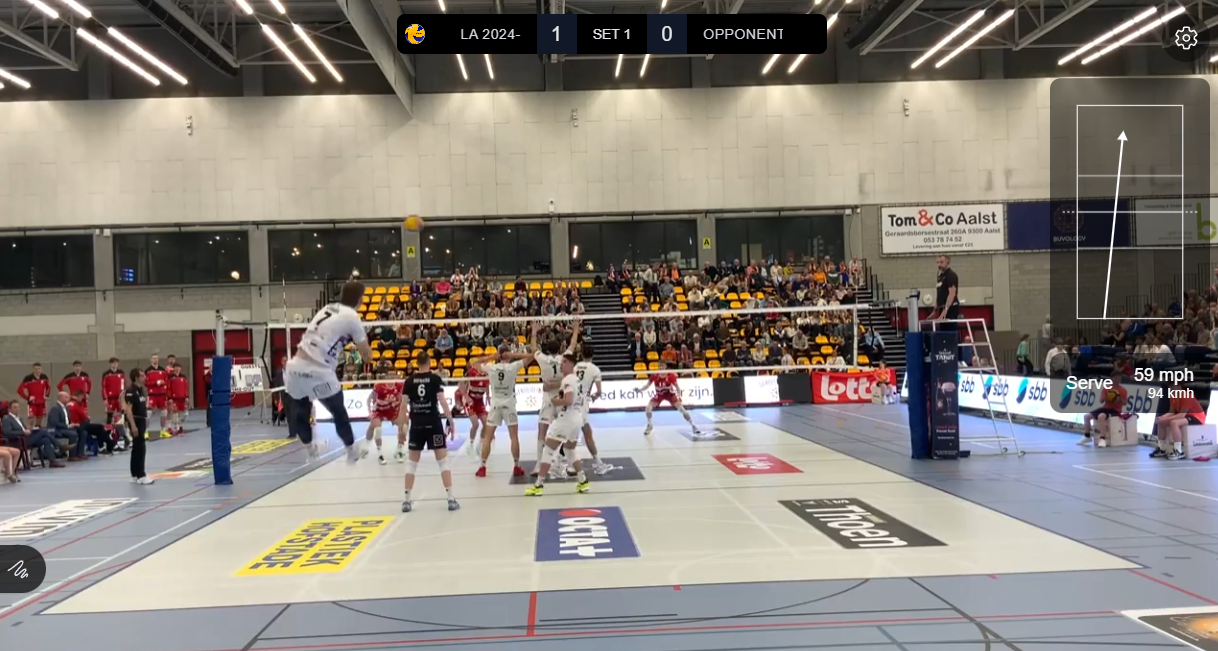
\includegraphics[width=\textwidth]{PL1_AM/opslag.png}
  \caption{\label{fig:PL1_Serve}Voorbeeld van opslagmeting van Balltime AI.}
\end{figure}

Ook in de tweede set, zie tabel \ref{tab:PL1ServeAI2}, valt op dat Balltime AI niet alle snelheden heeft opgemeten. In deze set zijn er 23 metingen gedaan van de 46 opslagen, 50\% van de opslagen. Dit is een verbetering ten opzichte van de eerste set, maar er zijn nog steeds veel snelheden die niet zijn gemeten. De snelheden die wel zijn gemeten, zijn ook hier weer verschillend van de manueel gemeten snelheden. Bij stand 10-9 werd manueel 80 km/u gemeten, terwijl Balltime AI 114 km/u registreerde. Een kleinere afwijking was dan wel weer te vinden bij stand 16-13, waar Balltime AI een snelheid van 41 km/u aangaf tegenover 45 km/u bij de manuele meting. Balltime AI gaf op sommige momenten wel veel hogere waardes, zoals 122 km/u bij 13-11, waar manueel slechts 55 km/u werd gemeten. In deze set lijken er ook enkele consistentere snelheden te zijn gemeten, zoals bij 1-0, waar manueel de meting 93 km/u aangaf en Balltime AI 94 km/u aangaf.

\begin{table}[ht!]
  \centering
  \scriptsize
  \begin{tabular}{|c|c|c|c|} \hline
    L.A.-G.M. & L.A. & G.M. & km/u \\ \hline
    0-0 &  & 19 & 116 \\
    1-0 & 7 & & 93 \\
    1-1 &  & 14 & 50 \\
    2-1 & 1 & & 51 \\
    3-1 & 1 & & 53 \\
    3-2 &  & 10 & 95 \\
    4-2 & 13 & & 89 \\
    4-3 &  & 15 & 71 \\
    5-3 & 9 & & 97 \\
    5-4 &  & 2 & 90 \\
    6-4 & 11 & & 82 \\
    6-5 &  & 4 & 61 \\
    7-5 & 14 & & 53 \\
    7-6 &  & 19 & 116 \\
    8-6 & 7 &  & 101 \\
    8-7 &  & 14 & 55 \\
    8-8 &  & 14 & 58 \\
    9-8 & 7 & & 60 \\
    9-9 &  & 10 & 106 \\
    10-9 & 13 & & 80 \\
    11-9 & 13 & & 95 \\
    12-9 & 13 & & 97 \\
    12-10 &  & 15 & 109 \\
    12-11 &  & 15 & 92 \\
    13-11 & 9 &  & 55 \\
    13-12 &  & 2 & 93 \\
    14-12 & 11 &  & 98 \\
    14-13 &  & 4 & 53 \\
    15-13 & 14 &  & 51 \\
    16-13 & 14 &  & 45 \\
    16-14 &  & 19 & 114 \\
    17-14 & 7 &  & 105 \\
    18-14 & 7 &  & 100 \\
    18-15 &  & 14 & 50 \\
    18-16 &  & 14 & 58 \\
    19-16 & 3 &  & 106 \\
    20-16 & 3 &  & 98 \\
    20-17 &  & 10 & 105 \\
    21-17 & 13 &  & 97 \\
    22-17 & 13 &  & 106 \\
    23-17 & 13 &  & 100 \\
    23-18 &  & 15 & 58 \\
    23-19 &  & 15 & 79 \\
    24-19 & 9 &  & 98 \\
    24-20 &  & 2 & 108 \\
    24-21 &  & 2 & 101 \\
    25-21 &  &  &  \\ \hline
  \end{tabular}
  \caption[Manueel gemeten opslagsnelheden tijdens set 2]{\label{tab:PL1ServeMan2}Manueel gemeten opslagsnelheden tijdens set 2.}
\end{table}

\begin{table}[ht!]
  \centering
  \scriptsize
  \begin{tabular}{|c|c|c|c|} \hline
    L.A.-G.M. & L.A. & G.M. & km/u \\ \hline
    0-0 &  & 19 & - \\
    1-0 & 7 & & 94 \\
    1-1 &  & 14 & 56 \\
    2-1 & 1 & & 55 \\
    3-1 & 1 & & 59 \\
    3-2 &  & 10 & - \\
    4-2 & 13 & & - \\
    4-3 &  & 15 & - \\
    5-3 & 9 & & - \\
    5-4 &  & 2 & 95 \\
    6-4 & 11 & & - \\
    6-5 &  & 4 & - \\
    7-5 & 14 & & 71 \\
    7-6 &  & 19 & - \\
    8-6 & 7 &  & 70 \\
    8-7 &  & 14 & 54 \\
    8-8 &  & 14 & 43 \\
    9-8 & 7 & & 73 \\
    9-9 &  & 10 & 92 \\
    10-9 & 13 & & 114 \\
    11-9 & 13 & & 109 \\
    12-9 & 13 & & 98 \\
    12-10 &  & 15 & - \\
    12-11 &  & 15 & 74 \\
    13-11 & 9 &  & 122 \\
    13-12 &  & 2 & - \\
    14-12 & 11 &  & - \\
    14-13 &  & 4 & 52 \\
    15-13 & 14 &  & 113 \\
    16-13 & 14 &  & 41 \\
    16-14 &  & 19 & - \\
    17-14 & 7 &  & - \\
    18-14 & 7 &  & 53 \\
    18-15 &  & 14 & 49 \\
    18-16 &  & 14 & - \\
    19-16 & 3 &  & - \\
    20-16 & 3 &  & - \\
    20-17 &  & 10 & - \\
    21-17 & 13 &  & 118 \\
    22-17 & 13 &  & - \\
    23-17 & 13 &  & - \\
    23-18 &  & 15 & - \\
    23-19 &  & 15 & - \\
    24-19 & 9 &  & 33 \\
    24-20 &  & 2 & - \\
    24-21 &  & 2 & - \\
    25-21 &  &  &  \\ \hline
  \end{tabular}
  \caption[Gemeten opslagsnelheden door Balltime AI tijdens set 2]{\label{tab:PL1ServeAI2}Gemeten opslagsnelheden door Balltime AI tijdens set 2.}
\end{table}

\section{Conclusie}
De vergelijking tussen de AI-gegenereerde statistieken en de handmatige invoer onthulde specifieke verschillen in registratie en beoordeling. Bij de opslagstatistieken gebruikt Balltime AI een numeriek scoresysteem en is minder kritisch dan de handmatige invoer met symbolen. Echter, bij deze statistieken kijkt de AI wel naar hoe de tegenstander omgaat met de opslag. Dit vormt geen probleem voor de staf van Lindemans Aalst, aangezien deze gegevens ook nog steeds bruikbaar zijn voor hun analyses. Dit is ook het geval voor de receptiestatistieken.

Bij de spelverdeling, aanvalstatistieken en verdedigingsstatistieken werd de kwaliteit niet beoordeeld door Balltime AI. De blokstatistieken hadden het grootste verschil. De AI gaf geen duidelijke indicatie van wie het blok uitvoerde, terwijl dit bij de handmatige invoer wel het geval was. Dit is een belangrijk aandachtspunt voor de verdere ontwikkeling van het AI-systeem, aangezien deze informatie cruciaal is voor de analyse van de prestaties van individuele spelers.

De opslagsnelheden werden door Balltime AI niet altijd geregistreerd, wat een beperking vormt voor de volledigheid van de gegevens. De snelheden die wel werden gemeten, vertoonden aanzienlijke variaties ten opzichte van de handmatige metingen. Dit wijst op een mogelijke inconsistentie in de nauwkeurigheid van de AI-registratie, maar de manuele invoer was ook niet altijd even consistent. De snelheden worden ook niet elke match manueel gemeten, waardoor hiervoor de AI wel een meerwaarde kan bieden. De meting van de snelheden bij Balltime AI was ook nog in een testfase.

%TODO: zeggen dat het bij training wel voordeel gaat hebben, maar dat het bij wedstrijden niet altijd even nuttig is
